\documentclass[conference,10pt]{IEEEtran}
\usepackage[utf8]{inputenc}
\usepackage{graphicx}
\usepackage{amsmath}
\usepackage{booktabs}
\usepackage{multirow}
\usepackage{xcolor}
\usepackage[hidelinks]{hyperref}
\hypersetup{colorlinks=true,linkcolor=blue!70!black,citecolor=blue!70!black,urlcolor=blue!70!black}
\usepackage{float}
\usepackage{caption}
\usepackage{subcaption}
\usepackage{array}
\usepackage{cite}

\title{Automated Industrial Environmental Compliance Monitoring\\Using Multi-Temporal Sentinel-2 Imagery and\\Machine Learning Classification}

\author{
\IEEEauthorblockN{Oishikk Nag\IEEEauthorrefmark{1}, [Author 2]\IEEEauthorrefmark{1}, [Author 3]\IEEEauthorrefmark{1}, [Author 4]\IEEEauthorrefmark{1}, [Author 5]\IEEEauthorrefmark{1}}
\IEEEauthorblockA{\IEEEauthorrefmark{1}Department of Computer Science and Engineering\\
Indian Institute of Information Technology, Dharwad, Karnataka 580009, India\\
\textit{Course: Machine Learning (Sem VII) \quad Instructor: Dr.\ Sunil C K}}
}

\begin{document}
\maketitle

\begin{abstract}
This paper presents an automated pipeline for monitoring environmental compliance in industrial zones using multi-temporal Sentinel-2 satellite imagery and supervised machine learning. We analyze two industrial areas in Bengaluru, Peenya and Whitefield, across a four-year period (2020--2024) to detect green cover reduction and unauthorized construction. Our system integrates programmatic data acquisition via the STAC API, spectral index computation (NDVI, NDBI), Random Forest classification with 97.7\% accuracy, and automated violation extraction with geo-coordinates. Results indicate significant green cover loss of 22.6\% (Peenya) and 27.8\% (Whitefield), with 55 geo-tagged violation zones identified. The system generates compliance reports suitable for pollution control board review.
\end{abstract}

\begin{IEEEkeywords}
Remote sensing, NDVI, change detection, land cover classification, Random Forest, Sentinel-2, environmental compliance, industrial monitoring
\end{IEEEkeywords}

\section{Introduction}

Industrial expansion in Indian metropolitan areas frequently occurs at the expense of mandated green belts and environmental buffers. The Karnataka State Pollution Control Board (KSPCB) requires industrial zones to maintain minimum green cover thresholds, yet manual monitoring through field inspections is infrequent and difficult to scale \cite{cpcb2021}. Satellite-based remote sensing offers a scalable alternative for continuous environmental surveillance.

This work addresses \textbf{Statement~3} of the ML course project: developing a system that utilizes GIS boundary data to identify factory premises, analyzes satellite imagery over time to detect green cover reduction and unauthorized construction, applies ML models for vegetation and land-use classification, and generates compliance reports with geo-tagged violation alerts.

Our contributions are: (1) an end-to-end automated pipeline from data acquisition to report generation, (2) a Random Forest classifier trained on spectral features achieving 97--99\% accuracy, and (3) a quantitative compliance assessment of two major Bengaluru industrial areas over the 2020--2024 period.

\section{Study Area and Data}

\subsection{Study Zones}

We selected two industrial areas in Bengaluru, Karnataka (Fig.~\ref{fig:beforeafter}):

\begin{itemize}
    \item \textbf{Peenya Industrial Area} (13.01--13.07\textdegree N, 77.48--77.56\textdegree E): One of the largest industrial estates in South Asia, covering approximately 40 km\textsuperscript{2}. Hosts manufacturing, electronics, and heavy industry units.
    \item \textbf{Whitefield} (12.95--13.01\textdegree N, 77.72--77.80\textdegree E): A rapidly urbanizing IT corridor with mixed industrial and residential development, approximately 25 km\textsuperscript{2}.
\end{itemize}

\subsection{Satellite Data}

We used Sentinel-2 Level-2A (L2A) surface reflectance imagery acquired from the Microsoft Planetary Computer via the SpatioTemporal Asset Catalog (STAC) API \cite{pc2023}. Two acquisition periods were selected during the dry season (January--March) to minimize cloud interference:

\begin{itemize}
    \item \textbf{T1 (Baseline):} March 2020. Cloud cover: $<$0.2\%
    \item \textbf{T2 (Recent):} March 2024. Cloud cover: $<$0.01\%
\end{itemize}

Six spectral bands were acquired: B02 (Blue, 490\,nm), B03 (Green, 560\,nm), B04 (Red, 665\,nm), B08 (NIR, 842\,nm), B11 (SWIR1, 1610\,nm), and B12 (SWIR2, 2190\,nm), along with the Scene Classification Layer (SCL) for cloud masking. Bands at 20\,m resolution (B11, B12, SCL) were resampled to 10\,m using bilinear interpolation. The total dataset comprises 11.6 million multispectral pixels across 28 GeoTIFF files.

\subsection{Boundary Data}

Industrial zone boundaries were obtained from OpenStreetMap as GeoJSON polygons to delineate the areas of interest, serving as a proxy for KGIS (Karnataka GIS) industrial boundary layers.

\section{Methodology}

\subsection{Preprocessing}

Raw bands were stacked into 7-band composites (B02, B03, B04, B08, B11, B12, cloud mask). Cloud and shadow pixels were masked using the SCL band, retaining only classes 2, 4, 5, 6, 7, and 11 as valid. Valid pixel coverage exceeded 99.8\% across all acquisitions.

\subsection{Spectral Index Computation}

Three spectral indices were computed for each time period:

\textbf{Normalized Difference Vegetation Index (NDVI):}
\begin{equation}
    \text{NDVI} = \frac{\rho_{\text{NIR}} - \rho_{\text{Red}}}{\rho_{\text{NIR}} + \rho_{\text{Red}}}
\end{equation}

\textbf{Normalized Difference Built-up Index (NDBI):}
\begin{equation}
    \text{NDBI} = \frac{\rho_{\text{SWIR1}} - \rho_{\text{NIR}}}{\rho_{\text{SWIR1}} + \rho_{\text{NIR}}}
\end{equation}

\textbf{New Built-up Index (NBI):}
\begin{equation}
    \text{NBI} = \frac{\rho_{\text{Red}} \times \rho_{\text{SWIR1}}}{\rho_{\text{NIR}}}
\end{equation}

\subsection{Change Detection}

Bitemporal differencing was applied: $\Delta\text{NDVI} = \text{NDVI}_{T2} - \text{NDVI}_{T1}$ and $\Delta\text{NDBI} = \text{NDBI}_{T2} - \text{NDBI}_{T1}$. Vegetation loss was identified where $\Delta\text{NDVI} < -0.15$, and new construction where $\Delta\text{NDBI} > 0.10$. These thresholds were selected based on established remote sensing literature \cite{zha2003}.

\subsection{ML Classification}

A Random Forest (RF) classifier was trained for pixel-level land cover classification into five classes: Dense Vegetation (NDVI $>$ 0.4), Sparse Vegetation (0.2 $<$ NDVI $\leq$ 0.4), Built-up (NDBI $>$ 0, NDVI $<$ 0.2), Bare Soil, and Water.

Training labels were generated via threshold-based rules applied to NDVI/NDBI values. Critically, the RF was trained on \textbf{raw spectral bands only} (B02--B12), not on the indices used for labeling, to avoid circular validation. The model used 100 decision trees, max depth of 15, balanced class weights, and was evaluated on a stratified 70/30 train-test split.

For comparison, unsupervised K-Means clustering ($k=5$) was also applied to the same feature space.

\subsection{Violation Extraction}

Connected component analysis was applied to the change mask to identify contiguous violation regions. For each region exceeding 10 pixels (1000~m\textsuperscript{2}), the centroid was computed and transformed from the image CRS (UTM 43N) to geographic coordinates (EPSG:4326) using PyProj.

\subsection{Risk Classification}

A rule-based risk score was assigned: \textit{HIGH} if green cover change $< -30\%$, \textit{MEDIUM} if $< -15\%$, and \textit{LOW} otherwise.

\begin{figure}[t]
    \centering
    \includegraphics[width=\linewidth]{../results/before_after_peenya.png}
    \caption{Temporal change analysis for Peenya Industrial Area. Top: true-color RGB composites (2020 vs.\ 2024). Bottom: NDVI heatmaps showing vegetation decline from 55.7\% to 33.1\% green cover.}
    \label{fig:beforeafter}
\end{figure}

\section{Results}

\subsection{Change Detection}

Table~\ref{tab:change} summarizes the change detection results. Both zones show significant green cover loss over the four-year period, with Whitefield showing more severe degradation.

\begin{table}[t]
\centering
\caption{Change Detection Results (2020--2024)}
\label{tab:change}
\begin{tabular}{lcc}
\toprule
\textbf{Metric} & \textbf{Peenya} & \textbf{Whitefield} \\
\midrule
Green Cover 2020 (\%) & 55.71 & 71.25 \\
Green Cover 2024 (\%) & 33.15 & 43.45 \\
Net Change (\%) & $-$22.56 & $-$27.80 \\
Vegetation Loss (\%) & 29.60 & 38.92 \\
New Construction (\%) & 4.59 & 17.72 \\
Violations Detected & 12 & 43 \\
Risk Level & MEDIUM & MEDIUM \\
\bottomrule
\end{tabular}
\end{table}

NDVI statistics confirm the trend: Peenya's mean NDVI dropped from 0.277 to 0.169, and Whitefield's from 0.353 to 0.218. Both zones remain above the HIGH-risk threshold but are approaching it.

\subsection{ML Classification}

Table~\ref{tab:ml} presents the Random Forest validation metrics. High accuracy ($>$97\%) was achieved across both zones, with the model effectively distinguishing five land cover classes using only raw spectral reflectance.

\begin{table}[t]
\centering
\caption{Random Forest Classification Metrics}
\label{tab:ml}
\begin{tabular}{lcc}
\toprule
\textbf{Metric} & \textbf{Peenya} & \textbf{Whitefield} \\
\midrule
Training Samples & 405,333 & 176,733 \\
Test Samples & 173,715 & 75,743 \\
Accuracy & 0.9774 & 0.9870 \\
Precision (weighted) & 0.9806 & 0.9879 \\
Recall (weighted) & 0.9774 & 0.9870 \\
F1-Score (weighted) & 0.9783 & 0.9873 \\
\bottomrule
\end{tabular}
\end{table}

\begin{figure}[t]
    \centering
    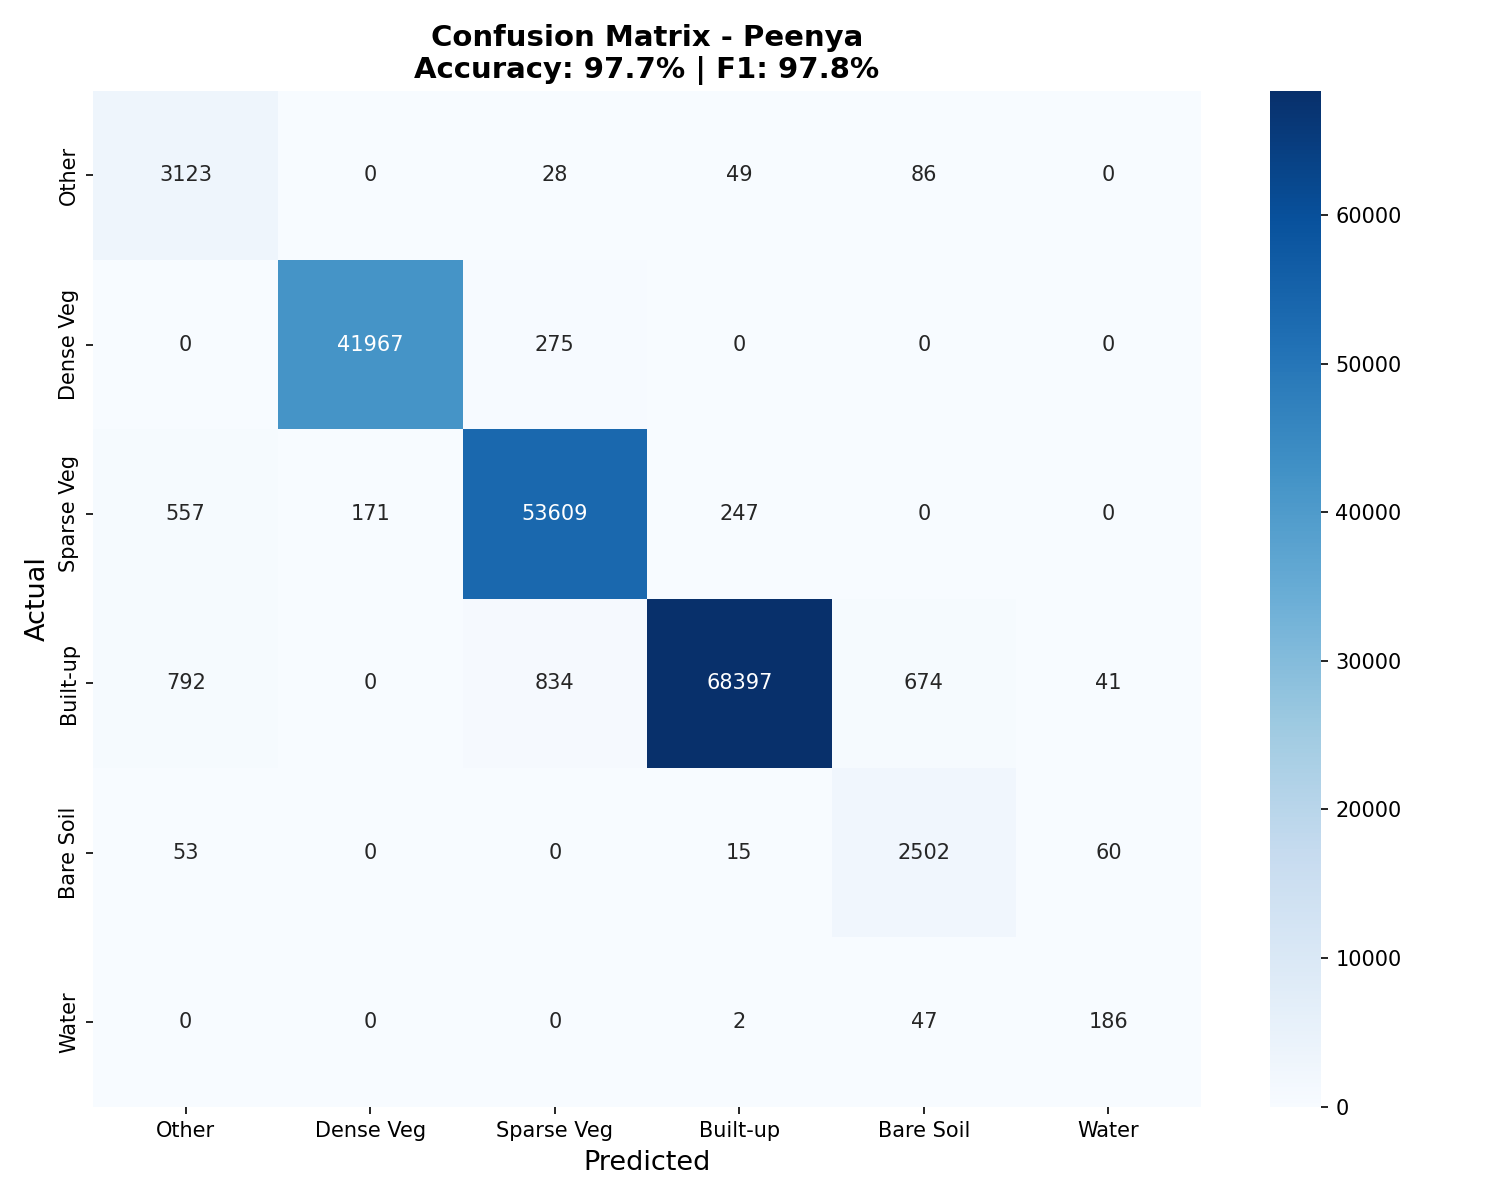
\includegraphics[width=\linewidth]{../results/confusion_matrix_peenya.png}
    \caption{Confusion matrix for Peenya RF classifier. Strong diagonal indicates high per-class accuracy. Minor confusion occurs between Bare Soil/Water and Other (minority classes).}
    \label{fig:cm}
\end{figure}

Fig.~\ref{fig:cm} shows the confusion matrix for Peenya. The three dominant classes (Dense Vegetation, Sparse Vegetation, Built-up) achieve F1-scores of 0.98--0.99. Minority classes (Water, Bare Soil) show lower but acceptable performance due to limited training samples.

Feature importance analysis (Fig.~\ref{fig:fi}) reveals that B04 (Red, 28.4\%) and B08 (NIR, 23.7\%) are the most discriminative bands. This is physically consistent, as the Red-NIR contrast forms the basis of NDVI and is the primary spectral signature distinguishing vegetation from non-vegetation surfaces \cite{tucker1979}.

\begin{figure}[t]
    \centering
    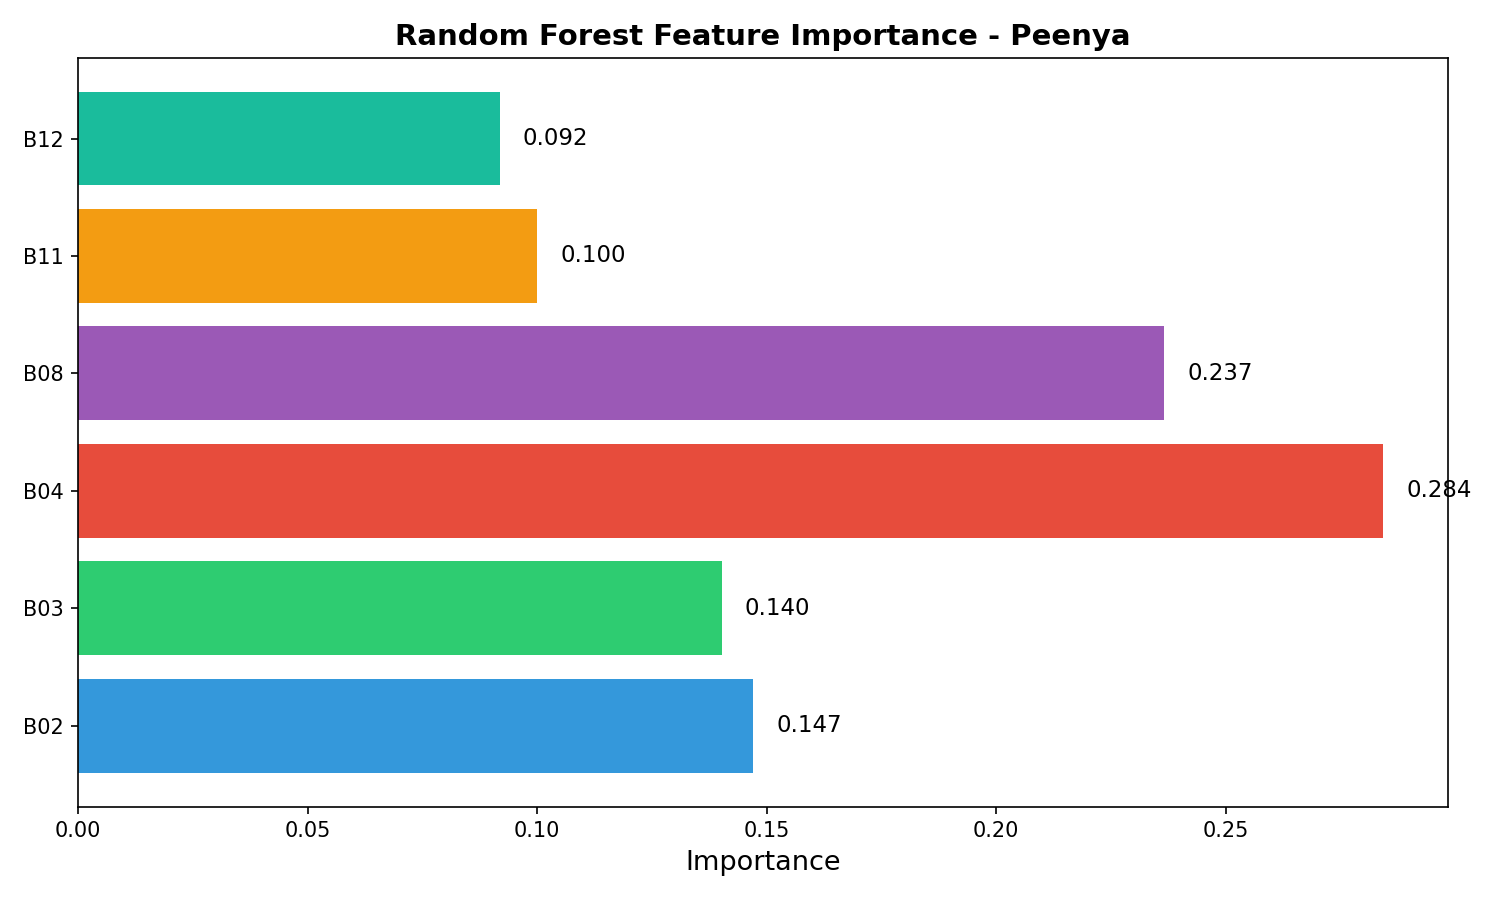
\includegraphics[width=\linewidth]{../results/feature_importance_peenya.png}
    \caption{Random Forest feature importance for Peenya. B04 (Red) and B08 (NIR) dominate, consistent with known vegetation spectral signatures.}
    \label{fig:fi}
\end{figure}

\subsection{Violation Detection}

A total of 55 violation zones were identified: 12 in Peenya and 43 in Whitefield. The largest vegetation loss region in Peenya spans 8.58 hectares centered at (13.069\textdegree N, 77.535\textdegree E). In Whitefield, combined vegetation loss and new construction hotspots were detected, the largest at 3.15 hectares (13.009\textdegree N, 77.731\textdegree E). Fig.~\ref{fig:violations} shows the annotated satellite imagery with geo-tagged violation markers.

\begin{figure}[t]
    \centering
    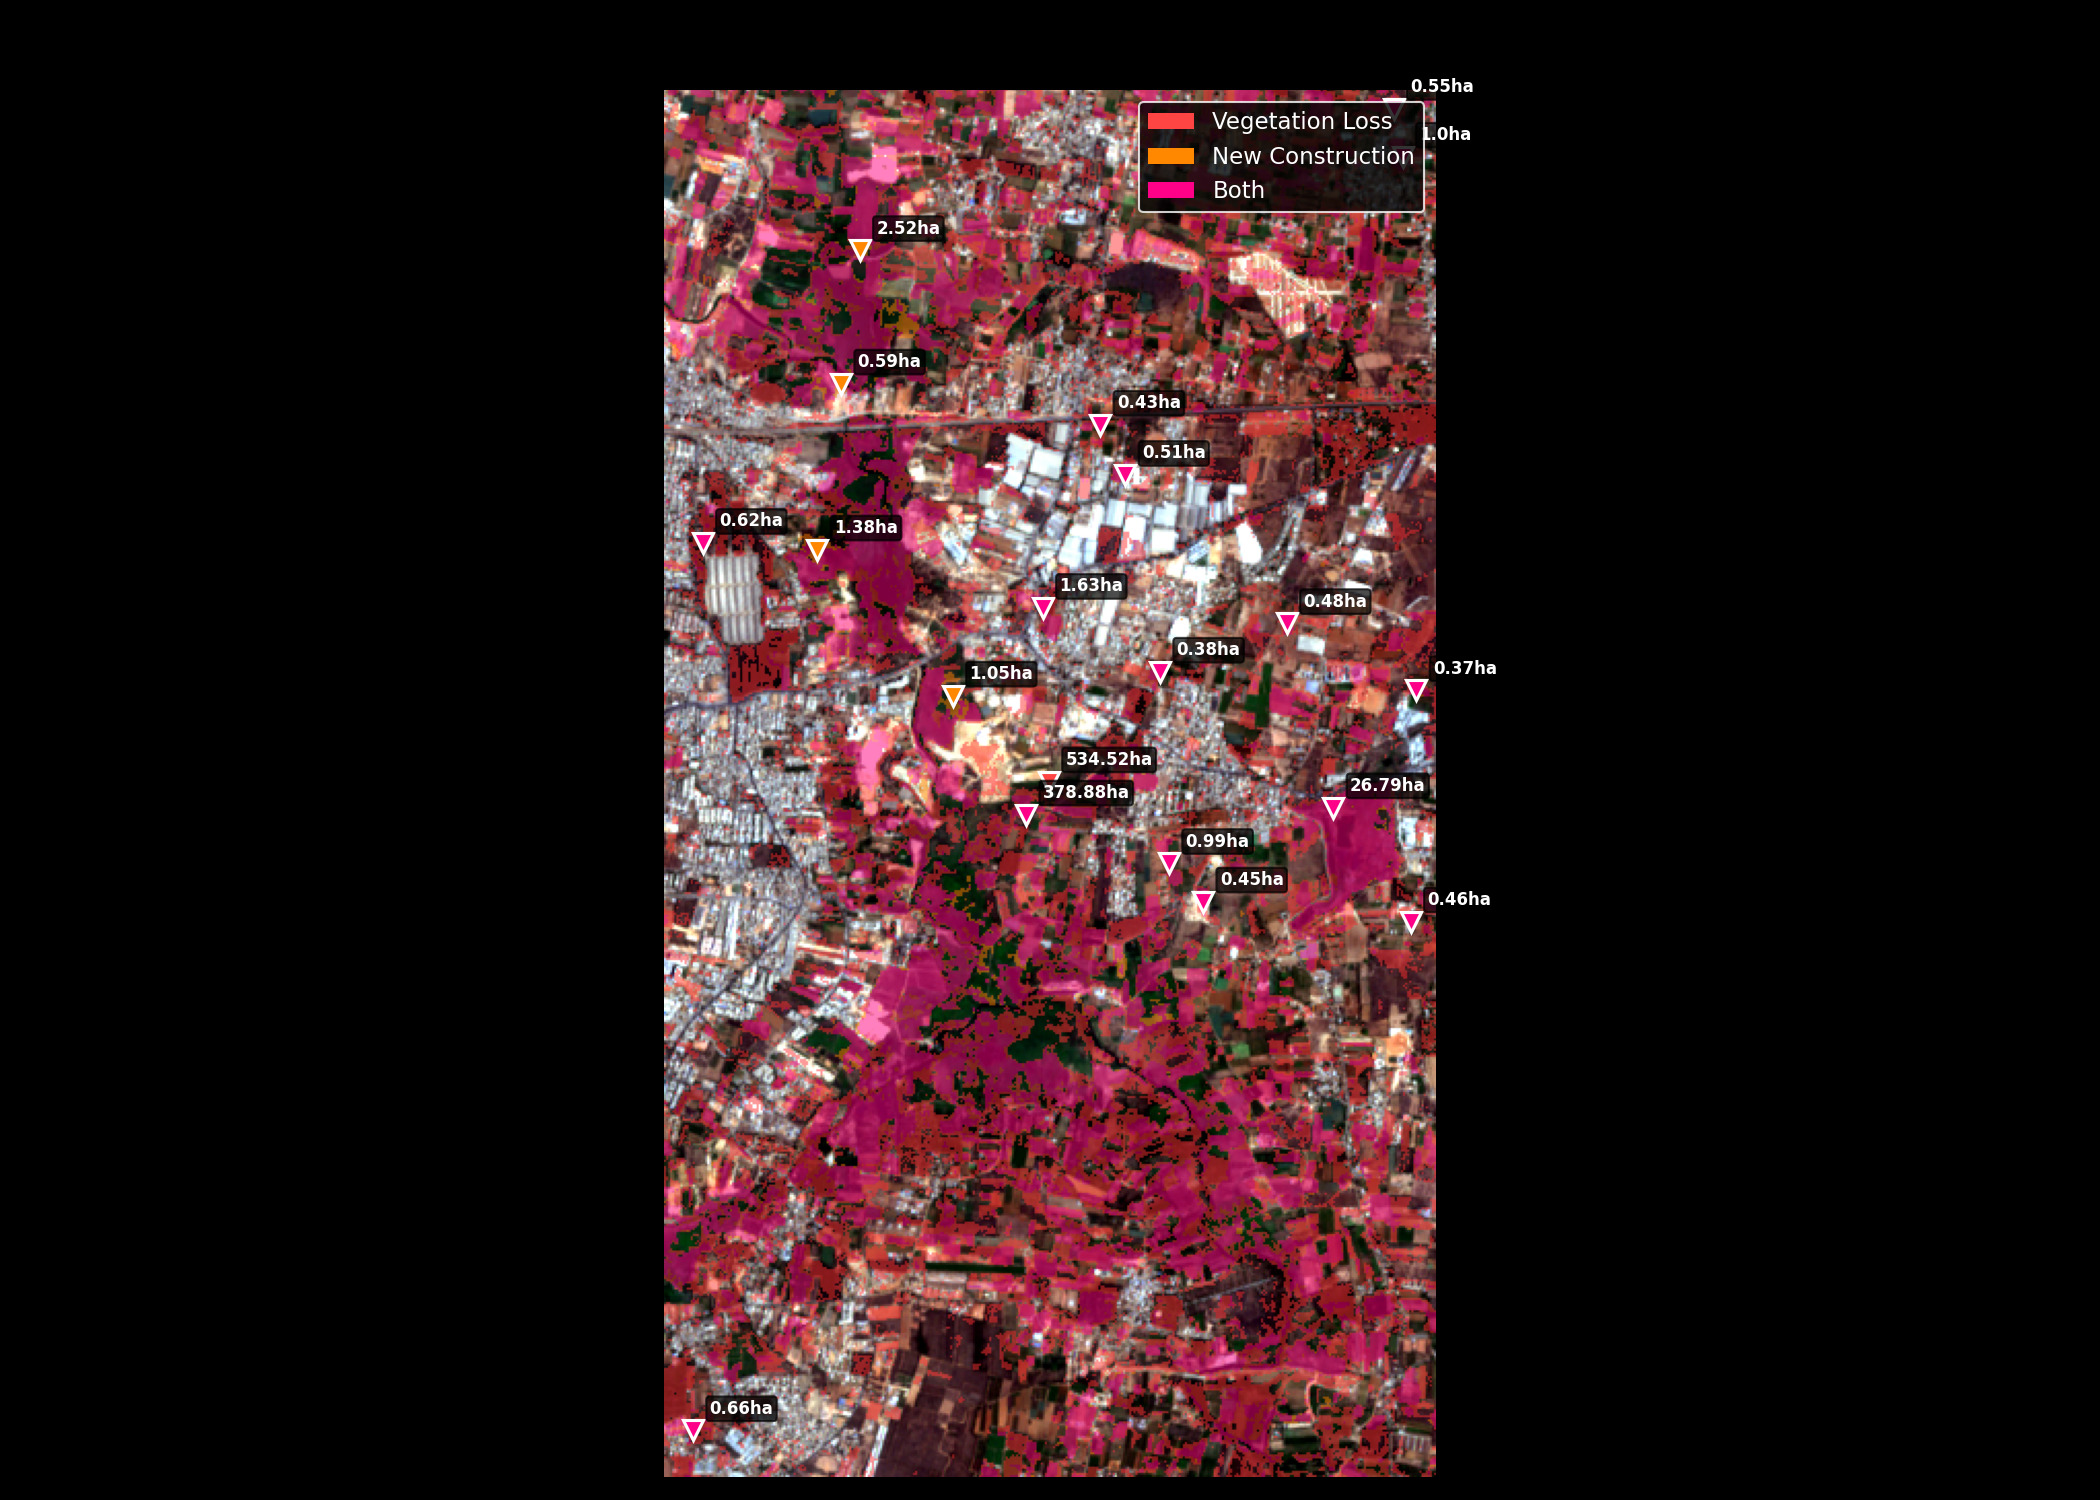
\includegraphics[width=\linewidth]{../results/annotated_violations_whitefield.png}
    \caption{Annotated satellite imagery of Whitefield showing detected violations with area labels. Red: vegetation loss, orange: new construction, pink: combined violations.}
    \label{fig:violations}
\end{figure}

\subsection{Land Cover Transition}

Fig.~\ref{fig:landcover} shows the ML-classified land cover maps for both time periods. The transition from dense/sparse vegetation (green) to built-up (brown) is clearly visible, particularly in the northern and eastern sectors of Peenya.

\begin{figure}[t]
    \centering
    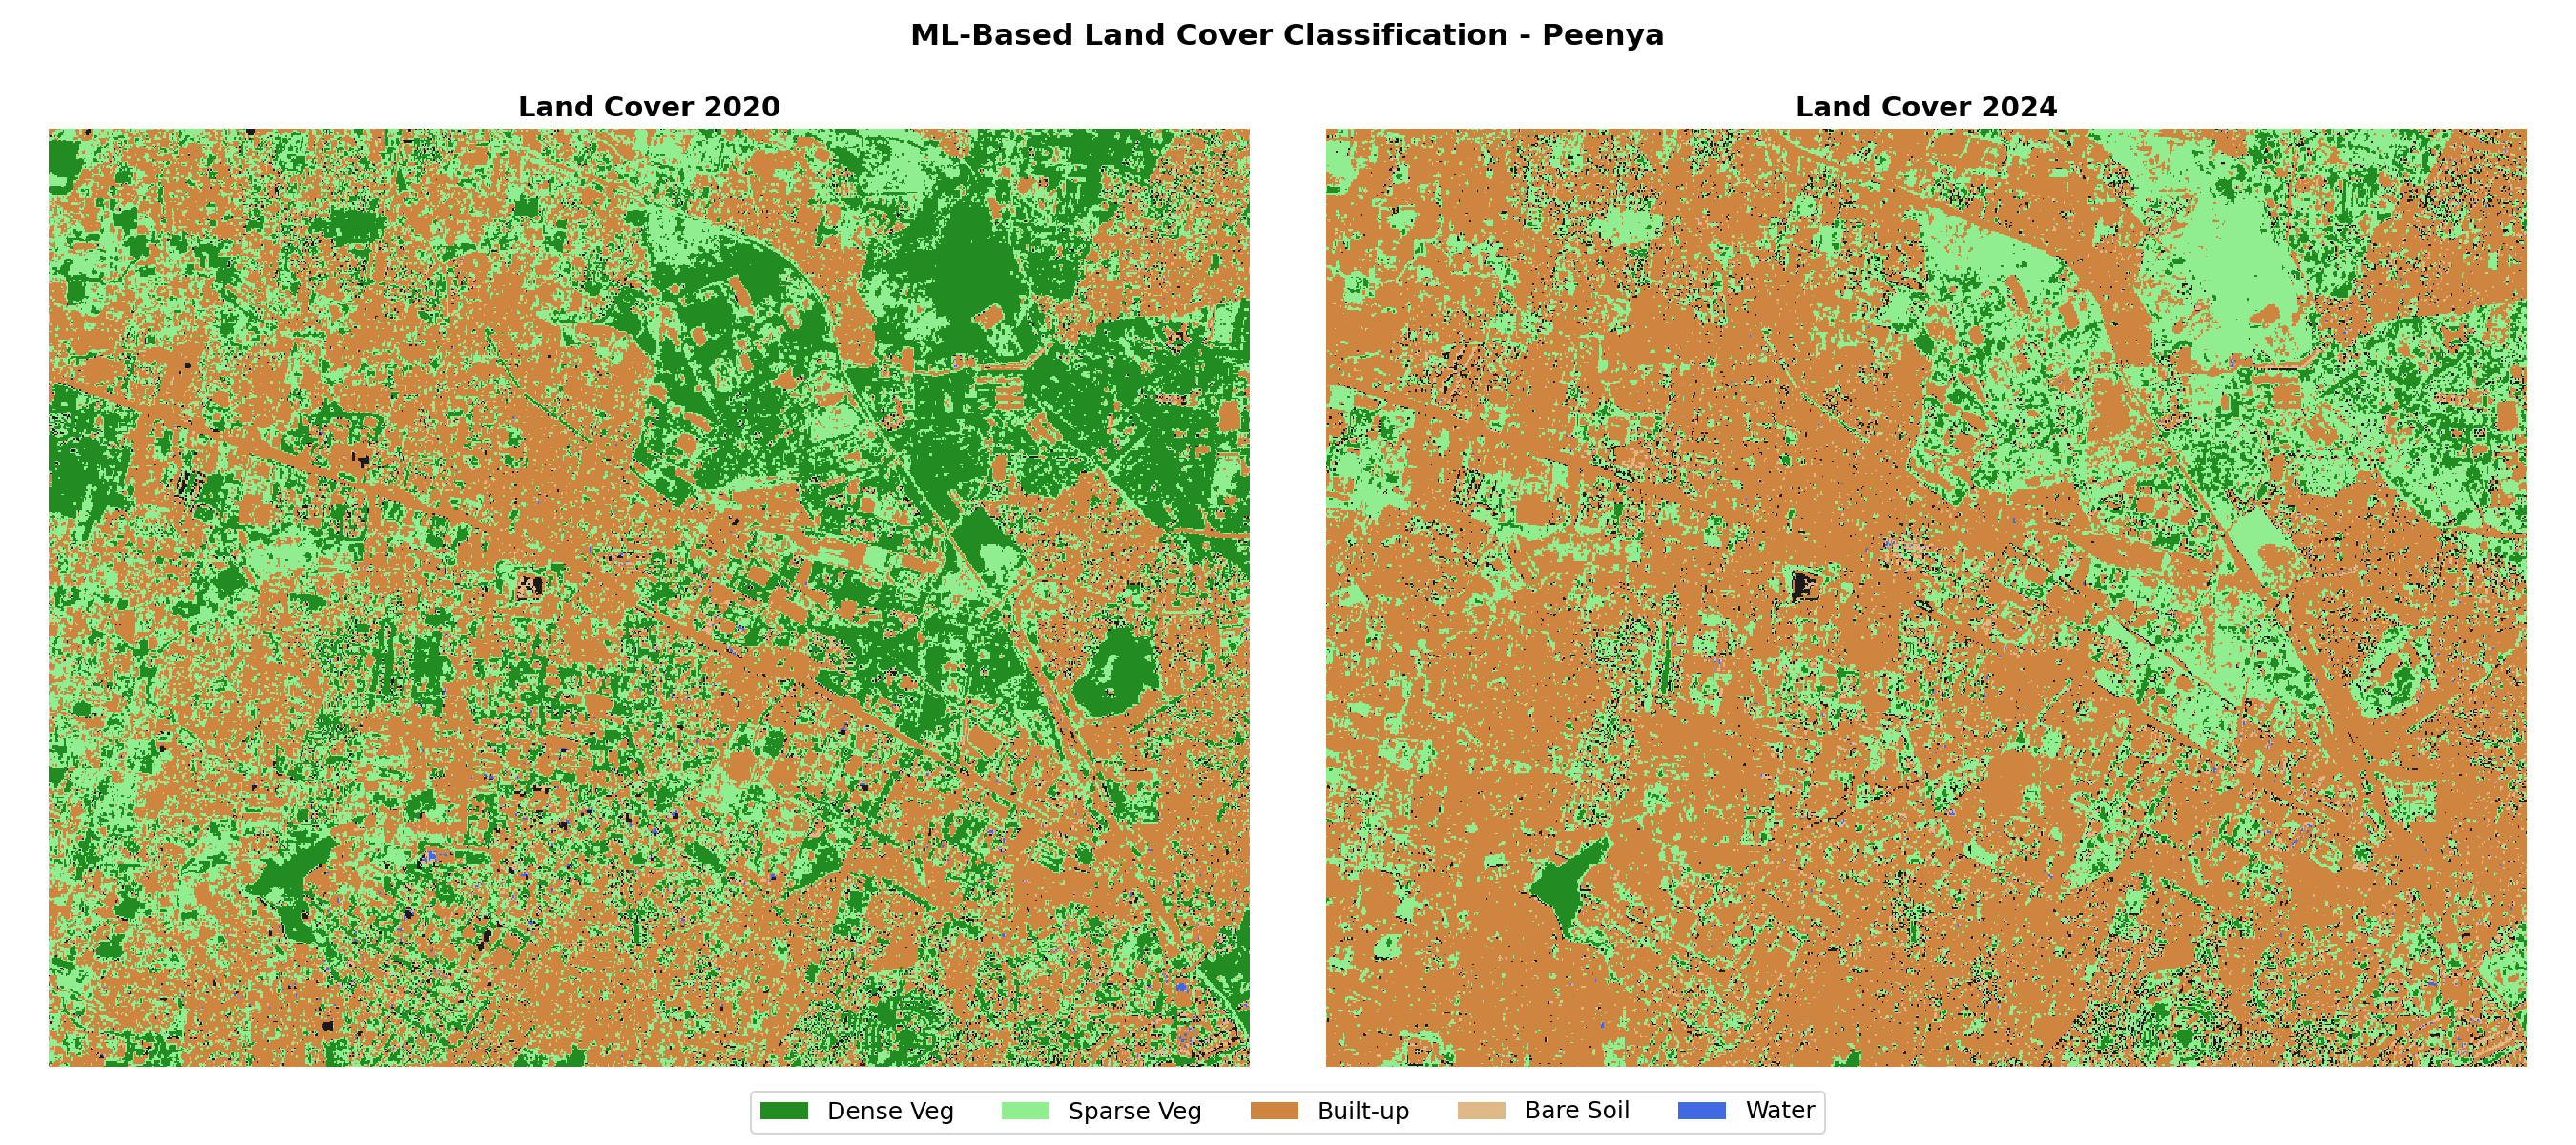
\includegraphics[width=\linewidth]{../results/landcover_comparison_peenya.png}
    \caption{Land cover classification comparison for Peenya (2020 vs.\ 2024). Green areas (vegetation) are visibly replaced by brown (built-up) across the study period.}
    \label{fig:landcover}
\end{figure}

\section{Discussion}

The detected green cover loss (22--28\%) across both industrial zones is concerning and aligns with publicly reported trends of rapid urbanization in Bengaluru's industrial corridors. Whitefield's higher new construction rate (17.7\% vs.\ 4.6\%) reflects the ongoing IT park and residential boom in that area.

The RF classifier's strong performance (97--99\%) validates the approach of using raw spectral bands for land cover classification. The non-circular validation design, where training features (raw bands) are independent of label sources (index thresholds), ensures that the reported metrics reflect genuine generalization capability.

A limitation of this study is the use of threshold-derived pseudo-labels rather than ground truth data from field surveys. Future work could incorporate KGIS cadastral data for parcel-level compliance assessment and deploy the system as a near-real-time monitoring service using Sentinel-2's 5-day revisit cycle.

\section{Conclusion}

We presented an automated pipeline for industrial environmental compliance monitoring that processes multi-temporal Sentinel-2 imagery to detect green cover loss and unauthorized construction. The system successfully identifies 55 violation zones across two Bengaluru industrial areas with geo-coordinates, achieves 97.7--98.7\% classification accuracy, and generates ready-to-use compliance reports. The modular design enables extension to any geographic region with minimal modification, supporting scalable environmental monitoring for pollution control boards.

\section*{Acknowledgment}

We thank Dr.\ Sunil C K for guidance on the project formulation. Satellite data was provided by the European Space Agency's Copernicus programme, accessed via Microsoft Planetary Computer.

\begin{thebibliography}{9}

\bibitem{cpcb2021}
Central Pollution Control Board, ``Guidelines for Environmental Compliance of Industrial Areas,'' Ministry of Environment, Forest and Climate Change, Government of India, 2021. [Online]. Available: \url{https://cpcb.nic.in}

\bibitem{pc2023}
Microsoft, ``Planetary Computer,'' 2023. [Online]. Available: \url{https://planetarycomputer.microsoft.com}

\bibitem{zha2003}
Y.~Zha, J.~Gao, and S.~Ni, ``Use of normalized difference built-up index in automatically mapping urban areas from TM imagery,'' \textit{Int.\ J.\ Remote Sensing}, vol.~24, no.~3, pp.~583--594, 2003.

\bibitem{tucker1979}
C.~J.~Tucker, ``Red and photographic infrared linear combinations for monitoring vegetation,'' \textit{Remote Sensing of Environment}, vol.~8, no.~2, pp.~127--150, 1979.

\bibitem{drusch2012}
M.~Drusch \textit{et al.}, ``Sentinel-2: ESA's optical high-resolution mission for GMES operational services,'' \textit{Remote Sensing of Environment}, vol.~120, pp.~25--36, 2012.

\bibitem{breiman2001}
L.~Breiman, ``Random Forests,'' \textit{Machine Learning}, vol.~45, no.~1, pp.~5--32, 2001.

\bibitem{rouse1974}
J.~W.~Rouse, R.~H.~Haas, J.~A.~Schell, and D.~W.~Deering, ``Monitoring vegetation systems in the Great Plains with ERTS,'' in \textit{Proc.\ Third Earth Resources Technology Satellite-1 Symp.}, vol.~1, pp.~309--317, 1974.

\bibitem{esa2024}
European Space Agency, ``Sentinel-2 User Handbook,'' ESA Standard Document, 2024. [Online]. Available: \url{https://sentinels.copernicus.eu/web/sentinel/user-guides/sentinel-2-msi}

\bibitem{pedregosa2011}
F.~Pedregosa \textit{et al.}, ``Scikit-learn: Machine Learning in Python,'' \textit{J.\ Machine Learning Research}, vol.~12, pp.~2825--2830, 2011.

\end{thebibliography}

\end{document}
